\section{Free Stationaries}
\begin{figure}[H]
    \centering
    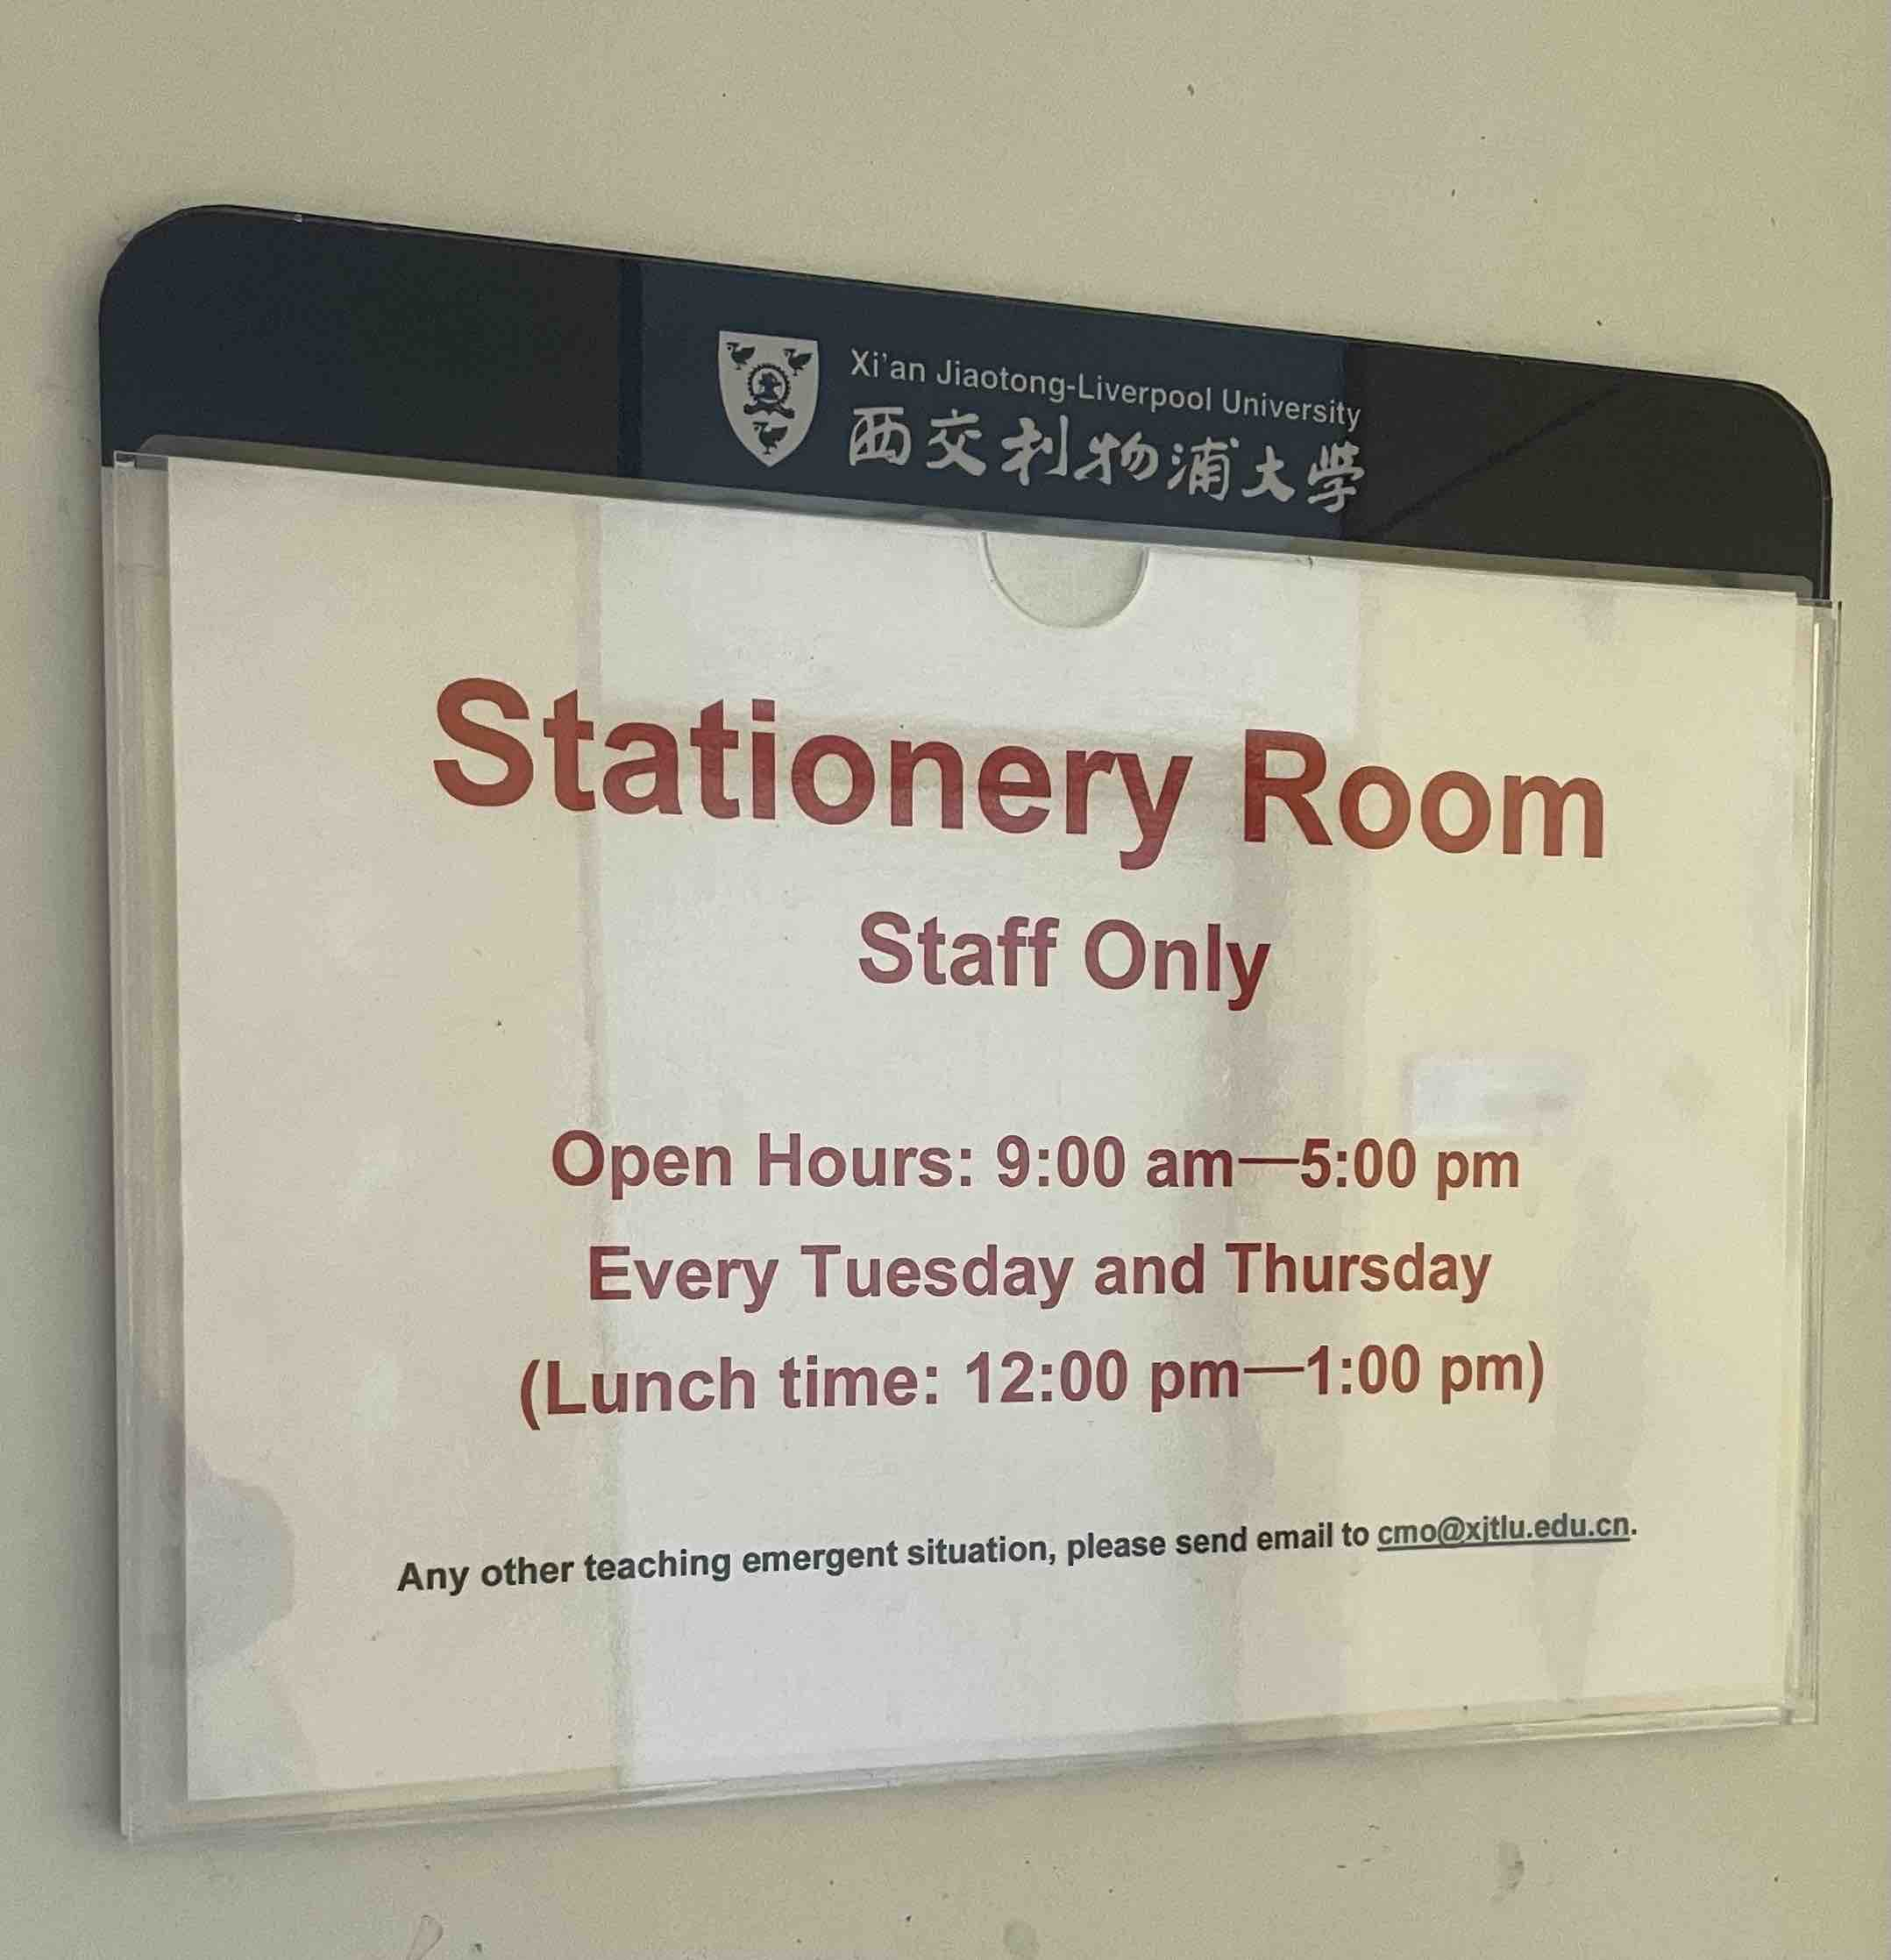
\includegraphics[width=0.6\columnwidth]{author-folder/Kai.Wu/stationery_room.jpg}
\end{figure}

Besides the substantial conference funds, the best way to save money is probably the free office supplies. Many buildings in the university have a Stationery Room (Office Supplies Collection Room), where all items are available for collection. Tissues, pens, markers, highlighters, various storage racks, tapes, glues, staplers—basically everything you can think of.

\vspace{5mm}
Locations of Stationery Rooms:
\begin{itemize}
    \item MB128, Tuesday/Thursday, 9–11 am, 1–5 pm
    \item BSG35, Tuesday/Thursday, 9–11 am, 1–5 pm (Thanks to an anonymous classmate for the addition)
    \item HS Building Property Office, Monday/Wednesday, 9–11 am, 1–5 pm, Friday morning (Thanks to an anonymous classmate for the addition)
    \item Other buildings? Please add
\end{itemize}

\hfill\break
How to collect:
\begin{enumerate}
    \item Before your first collection, go directly to the Stationery Room and ask the staff what items are available. They will give you a booklet. You can take photos of each page for reference, so you’ll know what you can get next time. Alternatively, you can find a historical version uploaded by a helpful classmate here \href{https://github.com/xp-pgrs-unofficial-guide/xp_pgrs_unofficial_guide/tree/main/fileshare}{[GitHub Link]} \href{https://gitee.com/kaiwu-astro/xp_pgrs_unofficial_guide/tree/main/fileshare}{[Alternate Link if you can't access GitHub]}, but the content may have slight differences due to changes.
    \item Download the latest (CMO) Office Supplies Application Form; the current latest version is V3. Old versions generally cannot be used after a new version is released. If this expires, where can we download the updated version? Unfortunately, we can't download it \sout{(complain about the university here)}; the usual method is to ask your supervisor, who can usually find it in the school's Box cloud storage. Here's the one I'm using \href{https://github.com/xp-pgrs-unofficial-guide/xp_pgrs_unofficial_guide/tree/main/fileshare}{Link} \href{https://gitee.com/kaiwu-astro/xp_pgrs_unofficial_guide/tree/main/fileshare}{Backup Link}.
    \item Fill in the form truthfully. The first column [Office Supplies Name] must exactly match the item names in the booklet mentioned above. You can't take too much at once; the staff will check. You can only take one box of tissues each time. Pens are generally taken individually, not by the box (but you can write down 12 pieces, which equals one box). For the reasons on the right, fill in truthfully and simply, such as Tissues—Daily Use; Pens—Calculations; Stapler—Organizing; Glue—Reimbursement. Finally, your supervisor needs to sign. Electronic signatures probably cannot be used, and you can't photocopy after your supervisor signs (these were common tricks in previous versions, haha). After filling it out, take it to the Stationery Room during open hours, and you can happily enjoy free shopping.
    \item Updated June 2023: The following items can be taken directly without filling out a form (others require the normal form)
\end{enumerate}

\begin{figure}[H]
    \centering
    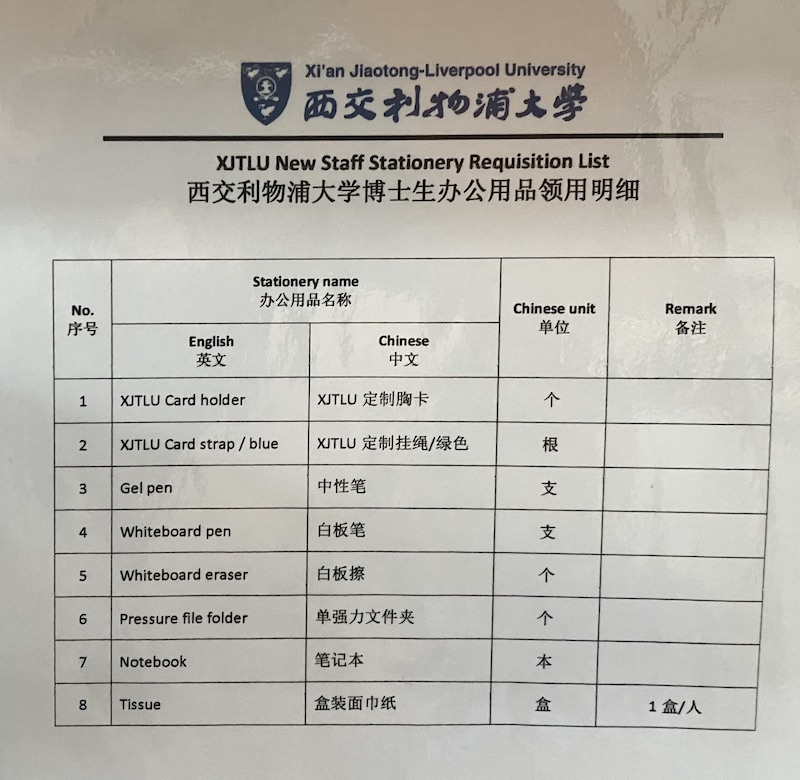
\includegraphics[width=0.6\columnwidth]{author-folder/Kai.Wu/stationery_no_sign.jpg}
\end{figure}

\begin{flushright}
    October 12, 2022 by \Wu \\
    GPT translation proofread by \Shiyao
\end{flushright}
